%% BioMed_Central_Tex_Template_v1.06
%%                                      %
%  bmc_article.tex            ver: 1.06 %
%                                       %

%%IMPORTANT: do not delete the first line of this template
%%It must be present to enable the BMC Submission system to
%%recognise this template!!

%%%%%%%%%%%%%%%%%%%%%%%%%%%%%%%%%%%%%%%%%
%%                                     %%
%%  LaTeX template for BioMed Central  %%
%%     journal article submissions     %%
%%                                     %%
%%          <8 June 2012>              %%
%%                                     %%
%%                                     %%
%%%%%%%%%%%%%%%%%%%%%%%%%%%%%%%%%%%%%%%%%


%%%%%%%%%%%%%%%%%%%%%%%%%%%%%%%%%%%%%%%%%%%%%%%%%%%%%%%%%%%%%%%%%%%%%
%%                                                                 %%
%% For instructions on how to fill out this Tex template           %%
%% document please refer to Readme.html and the instructions for   %%
%% authors page on the biomed central website                      %%
%% http://www.biomedcentral.com/info/authors/                      %%
%%                                                                 %%
%% Please do not use \input{...} to include other tex files.       %%
%% Submit your LaTeX manuscript as one .tex document.              %%
%%                                                                 %%
%% All additional figures and files should be attached             %%
%% separately and not embedded in the \TeX\ document itself.       %%
%%                                                                 %%
%% BioMed Central currently use the MikTex distribution of         %%
%% TeX for Windows) of TeX and LaTeX.  This is available from      %%
%% http://www.miktex.org                                           %%
%%                                                                 %%
%%%%%%%%%%%%%%%%%%%%%%%%%%%%%%%%%%%%%%%%%%%%%%%%%%%%%%%%%%%%%%%%%%%%%

%%% additional documentclass options:
%  [doublespacing]
%  [linenumbers]   - put the line numbers on margins

%%% loading packages, author definitions

%\documentclass[twocolumn]{bmcart}% uncomment this for twocolumn layout and comment line below
\documentclass{bmcart}

%%% Load packages
%\usepackage{amsthm,amsmath}
%\RequirePackage{natbib}
%\RequirePackage[authoryear]{natbib}% uncomment this for author-year bibliography
%\RequirePackage{hyperref}
\usepackage[utf8]{inputenc} %unicode support
%\usepackage[applemac]{inputenc} %applemac support if unicode package fails
%\usepackage[latin1]{inputenc} %UNIX support if unicode package fails

\usepackage{latexsym}
\usepackage{graphicx}
\usepackage{longtable}
\usepackage{amsmath}
\usepackage{mathtools}
\usepackage{booktabs}
\usepackage{fixltx2e}
\usepackage{multirow, makecell}
\usepackage{amssymb}
\usepackage{caption}
\usepackage{tikz}
\usepackage{url}
\usepackage{cuted}
\usepackage{lipsum}
\usepackage{float}

%%%%%%%%%%%%%%%%%%%%%%%%%%%%%%%%%%%%%%%%%%%%%%%%%
%%                                             %%
%%  If you wish to display your graphics for   %%
%%  your own use using includegraphic or       %%
%%  includegraphics, then comment out the      %%
%%  following two lines of code.               %%
%%  NB: These line *must* be included when     %%
%%  submitting to BMC.                         %%
%%  All figure files must be submitted as      %%
%%  separate graphics through the BMC          %%
%%  submission process, not included in the    %%
%%  submitted article.                         %%
%%                                             %%
%%%%%%%%%%%%%%%%%%%%%%%%%%%%%%%%%%%%%%%%%%%%%%%%%


% \def\includegraphic{}
% \def\includegraphics{}



%%% Put your definitions there:
\startlocaldefs
\endlocaldefs


%%% Begin ...
\begin{document}

%%% Start of article front matter
\begin{frontmatter}

\begin{fmbox}
\dochead{Research}

%%%%%%%%%%%%%%%%%%%%%%%%%%%%%%%%%%%%%%%%%%%%%%
%%                                          %%
%% Enter the title of your article here     %%
%%                                          %%
%%%%%%%%%%%%%%%%%%%%%%%%%%%%%%%%%%%%%%%%%%%%%%

% Min: too wordy.  Do you really need Neural? If no one else has done this task before use a shorter title
\title{Neural Side Effect Discovery from User Credibility and Experience-Assessed Online Health Discussions}
% \title{Neural Architecture-based Treatment Side Effect Prediction from Online User-generated Content and User Credibility Analysis}

%%%%%%%%%%%%%%%%%%%%%%%%%%%%%%%%%%%%%%%%%%%%%%
%%                                          %%
%% Enter the authors here                   %%
%%                                          %%
%% Specify information, if available,       %%
%% in the form:                             %%
%%   <key>={<id1>,<id2>}                    %%
%%   <key>=                                 %%
%% Comment or delete the keys which are     %%
%% not used. Repeat \author command as much %%
%% as required.                             %%
%%                                          %%
%%%%%%%%%%%%%%%%%%%%%%%%%%%%%%%%%%%%%%%%%%%%%%

%Kaz-JBMS: Please specify all of the author names. 
%Hoang-JBMS: Noted with thanks. I included all authors' details.
% \author[
%   addressref={aff1},                   % id's of addresses, e.g. {aff1,aff2}
%   corref={aff1},                       % id of corresponding address, if any
%   noteref={n1},                        % id's of article notes, if any
%   email={jane.e.doe@cambridge.co.uk}   % email address
% ]{\inits{JE}\fnm{Jane E} \snm{Doe}}
% \author[
%   addressref={aff1,aff2},
%   email={john.RS.Smith@cambridge.co.uk}
% ]{\inits{JRS}\fnm{John RS} \snm{Smith}}
\author[
   addressref={aff1},
   email={vhnguyen@u.nus.edu}
]{\fnm{Van-Hoang} \snm{Nguyen}}
\author[
   addressref={aff1},
   email={sugiyama@comp.nus.edu.sg}
]{\fnm{Kazunari} \snm{Sugiyama}}
\author[
   addressref={aff1},
   email={kanmy@comp.nus.edu.sg}
]{\fnm{Min-Yen} \snm{Kan}}

\author[
   addressref={aff1},
   email={kishaloy@comp.nus.edu.sg}
]{\fnm{Kishaloy} \snm{Halder}}

%%%%%%%%%%%%%%%%%%%%%%%%%%%%%%%%%%%%%%%%%%%%%%
%%                                          %%
%% Enter the authors' addresses here        %%
%%                                          %%
%% Repeat \address commands as much as      %%
%% required.                                %%
%%                                          %%
%%%%%%%%%%%%%%%%%%%%%%%%%%%%%%%%%%%%%%%%%%%%%%

\address[id=aff1]{%                           % unique id
  \orgname{School of Computing, National University of Singapore},
  \street{13 Computing Drive},
  \postcode{117417},
  \city{Singapore}
}
% \address[id=aff2]{%
%   \orgname{Marine Ecology Department, Institute of Marine Sciences Kiel},
%   \street{D\"{u}sternbrooker Weg 20},
%   \postcode{24105}
%   \city{Kiel},
%   \cny{Germany}
% }

%%%%%%%%%%%%%%%%%%%%%%%%%%%%%%%%%%%%%%%%%%%%%%
%%                                          %%
%% Enter short notes here                   %%
%%                                          %%
%% Short notes will be after addresses      %%
%% on first page.                           %%
%%                                          %%
%%%%%%%%%%%%%%%%%%%%%%%%%%%%%%%%%%%%%%%%%%%%%%

% \begin{artnotes}
% %\note{Sample of title note}     % note to the article
% \note[id=n1]{Equal contributor} % note, connected to author
% \end{artnotes}

\end{fmbox}% comment this for two column layout

%%%%%%%%%%%%%%%%%%%%%%%%%%%%%%%%%%%%%%%%%%%%%%
%%                                          %%
%% The Abstract begins here                 %%
%%                                          %%
%% Please refer to the Instructions for     %%
%% authors on http://www.biomedcentral.com  %%
%% and include the section headings         %%
%% accordingly for your article type.       %%
%%                                          %%
%%%%%%%%%%%%%%%%%%%%%%%%%%%%%%%%%%%%%%%%%%%%%%

\begin{abstractbox}

\begin{abstract} % abstract
% \parttitle{First part title} %if any
% Text for this section.

% \parttitle{Second part title} %if any
% Text for this section.
\parttitle{Background}
Health~2.0 allows patients and caregivers to conveniently seek medical information and advice via e-portals and online discussion forums, especially regarding potential drug side effects. While online health communities are helpful platforms for obtaining non-professional opinions, they pose risks in communicating unreliable and insufficient information in terms of quality and quantity. Existing methods in extracting user-reported adverse drug reactions (ADR) in online health forums are not only insufficiently accurate as they disregard author credibility and global drug experience, but are also expensive as they rely on supervised ground truth annotation at the statement level. 
We propose a NEural ArchiTecture for Drug side effect prediction (NEAT), which is optimized on a self-supervised prediction task of mentioned drugs' side effects at the discussion level that addresses these shortcomings. 
NEAT learns to assign each user a score that is descriptive of her credibility and highlights the critical textual segments of her post.

\parttitle{Results}
Experiments show that NEAT improves drug side effect discovery from online health discussion by 3.04\% from non-user-aware baselines and by 9.94\% from non-neural baselines in term of $F_1$. Additionally, output credibility scores statistically correlate with trustworthiness signals, such as number of ``thanks'' received by other forum members, and improve credibility heuristics such as number of posts by 0.113 in term of Spearman's rank correlation coefficient. Experience-based self-supervised attention highlights critical phrases such as mentioned side effects and enhances fully supervised ADR extraction models based on sequence labelling by 5.502\% in term of Precision.

\parttitle{Conclusions}
NEAT considers both users' reported content and global experiences in online health forums, making a self-supervised approach to side effect prediction for mentioned drugs feasible. The derived user credibility and attention mechanism are transferable and improve downstream ADR extraction models.
\begin{keyword}
\kwd{online health communities}
\kwd{drug side effect discovery}
\kwd{credibility analysis}
\kwd{deep learning}
\kwd{natural language processing}
\end{keyword}
\end{abstract}

%%%%%%%%%%%%%%%%%%%%%%%%%%%%%%%%%%%%%%%%%%%%%%
%%                                          %%
%% The keywords begin here                  %%
%%                                          %%
%% Put each keyword in separate \kwd{}.     %%
%%                                          %%
%%%%%%%%%%%%%%%%%%%%%%%%%%%%%%%%%%%%%%%%%%%%%%

% MSC classifications codes, if any
%\begin{keyword}[class=AMS]
%\kwd[Primary ]{}
%\kwd{}
%\kwd[; secondary ]{}
%\end{keyword}

\end{abstractbox}
%
%\end{fmbox}% uncomment this for twcolumn layout

\end{frontmatter}

%%%%%%%%%%%%%%%%%%%%%%%%%%%%%%%%%%%%%%%%%%%%%%
%%                                          %%
%% The Main Body begins here                %%
%%                                          %%
%% Please refer to the instructions for     %%
%% authors on:                              %%
%% http://www.biomedcentral.com/info/authors%%
%% and include the section headings         %%
%% accordingly for your article type.       %%
%%                                          %%
%% See the Results and Discussion section   %%
%% for details on how to create sub-sections%%
%%                                          %%
%% use \cite{...} to cite references        %%
%%  \cite{koon} and                         %%
%%  \cite{oreg,khar,zvai,xjon,schn,pond}    %%
%%  \nocite{smith,marg,hunn,advi,koha,mouse}%%
%%                                          %%
%%%%%%%%%%%%%%%%%%%%%%%%%%%%%%%%%%%%%%%%%%%%%%

%%%%%%%%%%%%%%%%%%%%%%%%% start of article main body
% <put your article body there>

%%%%%%%%%%%%%%%%
%% Background %%
%%

\section{Background}\label{sec:background}

Seeking medical opinions from online health communities has become commonplace: 71\% of adults aged 18--29 (equivalent to 59\% of all
U.S. adults) reported consulting online health
websites for opinions~\cite{fox2013health}.  These opinions come from an estimated
twenty to one hundred thousand health-related
websites~\cite{diaz2002patients}, inclusive of online health
communities that network patients with each other to provide
information and social support~\cite{johnston2013online}.  Platforms
such as
HealthBoards\footnote{\scriptsize{\url{https://www.healthboards.com/}}}
and MedHelp\footnote{{\scriptsize{\url{https://medhelp.ord/}}}}
feature users reporting their own health experiences, inclusive of
their self-reviewed drugs and medical treatments.  Hence, they are
valuable sources for researchers~\cite{leyens2017use,martin2014big}.

% Min: I think most journal prefer list citations [1,2,3] rather than separate citations [1][2][3].  Please check.
% Min: global replace as needed
Although patients use these platforms to access valuable information about drug reactions, there are challenges to their effective, large-scale use. There is lexical variation where users describe the same side effect differently.  For example, \textit{dizziness} can be expressed as
\textit{giddiness} or \textit{my head is spinning}, posing difficulty to most feature-based or keyword matching approaches. Separately there are valid concerns regarding credibility of user-generated contents to be harvested at large which research
has shown to be of variable quality and should be approached with caution~\cite{impicciatore1997reliability,peterson2003consumers,hajli2015credibility}. One proxy indicator for information quality is the author's trustworthiness~\cite{li2016survey}. In the context of social media or online forums, user trustworthiness is 
often approximated via ratings from other users, \textit{i.e.,} number of thanks or upvotes~\cite{rains2009health}, or via her consistency of reporting credible information~\cite{hoang2018authenticity,mukherjee2014people}. In addition to credibility, forum members also offer expertise thanks to their own experience -- with prescriptions in particular -- and facilitate responses to drug queries~\cite{vydiswaran2019identifying}. For instance, while reporting expected side effects for a specific treatment, patients with long-term use of certain drugs can be a complementary source of information:  %{\it E.g.}:

{\footnotesize
{\it While my experience of 10 years is with Paxil, I expect that Zoloft will be the same. You should definitely feel better within 2 weeks. One way I found to make it easier to sleep was to get lots of exercize [sic]. Walk or run or whatever to burn off that anxiety.} -- User 3690.
}

The above is an answer to a thread asking for expected side effects for
depression treatment with Zoloft. User 3690's history of active
discussion on other anti-depressants such as Lexapro and Xanax lends credibility to her being an authority on depression treatments. We noticed that Zoloft (mentioned in the thread) shares many common side effects with the other two anti-depressants: ``\textit{changed behavior},'' ``\textit{dry mouth},'' and ``\textit{sleepiness or unusual
drowsiness}.'' as illustrated in 
% Min: usually numbered artifacts are capitalized ``Table~1'', ``Section~2''
Table~\ref{table:anti_depressant_side_effects}. Many of such examples suggest that drugs which are often prescribed together for the same treatment, such as anti-depressants, are likely to be discussed within a same thread and share common side effects. In addition, users who have experienced certain reactions are opinionated and authoritative on those discussions involved drugs of similar side effects. These signals arise from the rich context of online health information, hence, we expect systems to explore beyond individual statements by considering the thread content as a whole as well as the global experience of each involved users, in order to discover drug side effects or extracting 
%Kaz2: It is better to specify what "ADRs" are as it first appears in the body of the paper while it is shown in "Abstract."  
%ADRs 
%Hoang2: noted with thanks
adverse drug reactions (ADRs) from online users.

We argue that modeling user expertise from previously experienced side effects is more robust compared to general user profile and engagement features~\cite{mukherjee2014people,vydiswaran2019identifying} as their expertise provides more meaningful signals for side effect discovery.
% Min: can you say this more strongly?
% Hoang: noted with thanks
To the best of our knowledge, there is no previous work that incorporates user expertise in side effect discovery in discussion forums at either the thread or post level.
In this work, given discussions in online health communities, we propose a novel end-to-end neural architecture that jointly models each author's credibility, her global experience and her post's textual content to discover the side effect of unseen drugs.
We optimize the model on a self-supervised task of predicting for side effect of mentioned drugs, where ground truth is accessible.  
Our key observation is that users can be grouped into clusters 
that share the same expertise or interest in certain drugs, 
possibly due to their common treatment or medical history. 
We incorporate this critical observation into our user model in representing a post's content via a cluster-sensitive attention mechanism~\cite{halder2018cold}.
We also follow general definition of truth discovery and let the
model learn a credibility score that is unique to every user and
descriptive of her trustworthiness.
Our experiments include an overall ablation study to validate the significance of the improvements garnered by each model component. Our proposed approach extends 
our former work~\cite{nguyen-etal-2018-treatment}  
by conducting a correlation study that analyzes the representativeness of 
credibility scores obtained by self-supervised learning  
as well as a comparison of our attention-based side effect mention extraction and sequence labeling approaches.

We summarize our contributions as follows: 
\begin{itemize}
% Min: global-- try to drop modal verbs to have more straightforward writing -- assess any ``would'' ``could'' ``should'' ``can'' and remove if possible
\item We propose a NEural ArchiTecture, NEAT, that captures user expertise and credibility, the semantic content of individual posts and the holistic thread to improve side effect discovery from online health discussions.
\item We formulate a self-supervised task of side effect prediction of mentioned drugs for the proposed network to jointly optimize its components.
\item We conduct experiments to verify the validity of our learned credibility and the robustness of self-supervised attention-based extraction, comparing against fully supervised sequence labeling baselines.
\end{itemize}

\section{Related Work}\label{sec:related_work}

We review the related work as per our listed contribution. We first review existing approaches to drug side effect discovery from health forums and social media. Next, we examine how these works incorporate user credibility and expertise in their learning objective. Finally, we justify our choice of neural architecture by discussing its modeling capability of context-rich structures such as online discussion. \\

{\bf Drug Side Effect Discovery.} Existing methods for drug discovery from online content extract drugs at post and statement level. ADR mining systems typically include 
a named entity recognition~(NER) model and a relationship or semantic role labeling model~\cite{sampathkumar2014mining,liu2018patient}. 
%Kaz2: Here, author names are not referred to. So the citation marks should be at the last of the sentence. 
%Recent neural approaches~\cite{ding2018attentive,wunnava2019adverse} 
Recent neural approaches address lexical variation in user-generated content -- the difficulty faced by traditional keyword matching and rule-based approaches -- to improve recognition and labeling components~\cite{ding2018attentive,wunnava2019adverse}. However, supervised sequence labeling or mention extraction approaches require laborious annotations at the word (token) level, and are only capable of discovering side effects that are explicitly present in the text. Expert supervision or additional semantic matching models are also required to map such recognized text segments to standardized vocabulary or thesaurus~\cite{yates2015extracting}. In contrast, our proposed self-supervised task formulation discovers the aggregated side effects of mentioned drugs for each community discussion by considering the whole thread's content. The list of discussed drugs are tagged by forum moderators or obtained by pattern matching. This learning design not only effectively alleviates the need for expensive, finer-grained annotations but also allows for the prediction of side effects not explicitly mentioned in the discussion. \\

{\bf User Credibility and Expertise Integration.}
% Min: what do you exactly mean by truth discovery?  Is that a technical term that is used here?
% Hoang: I have cited the papers on the concept of truth discovery
Credibility is of the utmost concern in large scale knowledge harvesting~\cite{hajli2015credibility,mukherjee2015leveraging,popat2016credibility}. Previous works on side effect discovery from individual statement or post derive information credibility by verifying a statement's mentioned side effects against ground truth drug-side effect databases, and user credibility by measuring the percentage of her credible statements~\cite{mukherjee2014people,li2017reliable}. Our approach to side effect discovery from discussion content by jointly model multiple posts and their authors does not derive statement credibility and derives user credibility differently. We assign each user a positive score that is used to weight her post content in representing the discussion's holistic content. Such weighted summation is mathematically shown in the Appendix to conform to the general principle of truth discovery, where sources providing credible information should be assigned higher credibility scores, and the information that is supported by credible sources will be
regarded as true~\cite{li2016survey}. Although our dataset does not provide any ground truth for user trustworthiness, we followed the previous usage of ratings or upvotes in online forums and adopted number of ``thanks'' received from other forum members~\cite{rains2009health} as our proxy for user trustworthiness. Previous works have modeled user expertise based on user profiles such as demographics; activity features such as posting frequency and posting pattern through time series and network analysis~\cite{mukherjee2014people, vydiswaran2019identifying}. As shown in an earlier example in section~\ref{sec:background}, modeling user expertise from previously experienced side effects better captures author authoritativeness for certain side effects and is universally applicable to any online platform. \\

{\bf Modeling Online Discussion Content and Structure}
% Min: what objects do you mean?
% Min: somehow the way you structure related work doesn't sit very well with me.  It lacks some of the big picture ideas before diving into details.
As our work makes use of the rich topographical properties of online communities, it also helps to briefly review approaches for modeling textual content and post-thread discussion structure. Previous works use probabilistic graphical models implicitly to represent textual content (especially, topic modeling) as bag-of-words~\cite{yates2015extracting}~\cite{wang2014sideeffectptm} or stylistic or linguistic features~\cite{mukherjee2014people}.
% Previous works which made use of Topic Modeling and Probabilistic Graphical Models implicitly represent textual content as bag-of-words~\cite{yates2015extracting}~\cite{wang2014sideeffectptm} or stylistic or linguistic features~\cite{mukherjee2014people}. 
% Min: ``moderate'' and ``rich'' in terms of what?  Size / length? Structure?
% Hoang: noted with thanks
Such lightweight representation are well-suited in moderately short contexts, \textit{i.e.,} sentences or posts. However, in terms of modeling long discussions consisting of multiple posts, state-of-the-art models for
% Min: Is Community Question Answering abbreviated as CQA or CoQA?  I've seen both. 
Community Question Answering feature hierarchical neural architectures~\cite{qiu2015convolutional,zhou2018recurrent,zhang2017attentive}. In term of encoding text, sequential encoders such as 
%Kaz2: Need to specify references for LSTM and CNN
Long Short-Term Memory (LSTM)~\cite{hochreiter1997long} or Convolutional Neural Networks (CNN)~\cite{kim2014convolutional} are capable of encoding long-term dependencies and semantic expressiveness by leveraging word embeddings. In terms of encoding hierarchical structures such as community discussions consisting of post- and thread-level features, neural architectures allow for straightforward and efficient integration of multiple learning objectives. In addition, our neural architecture, NEAT, incorporates attention mechanism that focus on essential phrases while encoding post content, and joint user credibility learning while optimizing for the side effect discovery objective.

%%%%%%%%%%%%%%%%%%%%%%%%%%%%%%
\section{Methods}\label{sec:proposed_method}

{\bf Basic Terminology.} To ensure a consistent representation, 
%Kaz2: Rewrite the following sentence as follows: 
%let us first define some terminology:
we first define some terminologies: 

\begin{itemize}
% Kishaloy: list => set
\item A \textit{drug d} has a set of side effects, \\
  $S_d = \{s_1, s_2, \ldots\}$
% Kishaloy: set => sequence
%Kaz-JBMS: I think that the following expression is better. 
%\item A \textit{post $p$} is the most basic document, containing a sequence of sentences. It is written by a \textit{user $u$}, and belongs to a \textit{thread $t$}.
% Hoang-JBMS: I agree. Noted with thanks.
\item A \textit{post $p$} is a message in online forums and contains a sequence of words. Post $p$ is written by a \textit{user $u$} and belongs to a \textit{thread $t$}.
\item A \textit{user $u$} is a member of an online community. He/She participates in a list of threads, \textit{ i.e., $T_u = \{t_1, t_2, \ldots, t_l\}$} by writing at least one post in each thread.
We use the terms \textit{user} and \textit{author}, as well as \textit{user experience} and \textit{user expertise} interchangeably.
\noindent
Each user is characterized by her credibility and expertise. Credibility $w_u$ of user $u$ reflects the probability of user $u$ provide trustworthy or helpful information, and is approximated from the number of ``thanks'' given from other forum members.

\item A \textit{thread t}
(see Table~\ref{table:sample_thread}) 
is an ordered collection of post--user pairs, 

$Q_t = [\left(p_1, u_1\right), \left(p_2, u_2\right), \ldots, \left(p_n, u_n\right)]$. 

\noindent
Every thread discusses the treatment for a particular condition and entails a list of prescribed drugs 
%\textit{$D_t = \{d_1, d_2 \cdots d_m\}$}. 
$D_t=\{d_1, d_2, \ldots, d_m\}$. 
Hence, every thread has a list of aggregated potential side effects defined as $S_t = S_{d_1} \cup S_{d_2} \cdots \cup S_{d_m}$. \\

\end{itemize}

% Min: BUG: Global: is it ``side effect'' or ``side-effect''?  Use
% just one.
% Hoang: noticed with thanks and replace all to side effects
{\bf Task Definition.} 
%Kaz2: "during" seems to be redundant. So I removed "during" and kept "from"
%{\it Drug side effect discovery during from discussions} 
{\it Drug side effect discovery from discussions} 
is the task of assigning the most relevant subset of potential
side effects to threads discussing certain drugs, from a large
collection of side effects. We view the drug side effect
discovery problem as a multi-label classification task. In our
setting, an instance of item--label is a tuple
$\left(\boldsymbol{x}_{t},\boldsymbol{y}\right)$ where
$\boldsymbol{x}_{t}$ is the feature vector of thread $t$ derived from
its list of
post--user pairs $Q_{t}$
and $\boldsymbol{y}$ is the side effect label vector \textit{i.e.}, $\boldsymbol{y}\in\{0, 1\}^S$, where $S$ is the number of possible side effect labels. Given training instances, we train our classifier to predict the list of drug side effects in unseen threads discussing unseen drugs. \\
% Kishaloy: BUG: T is already used to denote a thread. Can we use something else? Or maybe just drop the notation for number of instances.
% Hoang: Noticed and agreed, I dropped the notation

% Min: agreed.  Skip
%% This problem can be formally defined as follows: 
%% %Kaz: You may be able to skip the following as it is well-known framework on 
%% % supervised learning. 
%% \textit{Find a mapping $f : T \to \{0,1\}^{|S|}$ T is the set of all threads, S is the set of possible side effects, $f$ would give us a probability score for each of side effect $s_i$ given $\boldsymbol{x_t}$}
%% \begin{equation}
%% f(\boldsymbol{x_t}) = P(s_i=1|\boldsymbol{x_t}), 
%% \end{equation}
%% \textit{where $i \in \{1, 2, \ldots, |S|\}$, and $s_i$ is the label corresponding to $i^{th}$ side effect.}
% Hoang: noticed with thanks

%Kaz: You can just write $Q_t$ as it has already been defined in "Basic Terminologies".
% Kishaloy: This paragraph can be skipped IMO. Doesn't give any new information.
% Hoang: I think we should put forth a hypothesis which is the premise of our work. The results from our experiment would confirm this hypothesis and make the work cohesive
{\bf Formal Hypothesis.} Given a thread $t$ with $Q_t$, 
%$Q_t = \{\left(p_1, u_1\right), \left(p_2, u_2\right), \ldots, \left(p_n, u_n\right)\}$, 
we hypothesize that considering the credibility and experience of user $u \in \left(p, u\right) \in Q_t$ improves the quality of feature representation in thread $t$, resulting in better drug side effect discovery performance. \\

%Kaz: It is better to use "\boldsymbol{...}" to represent a vector or matrix. 
% See the first sentence at "User Expertise Representation" 
% Hoang: noticed with thanks
%%%%%%%%%%%%%%%%%%%%%%%%%%%%%%%%%%%%%%%%%%%%%%%%%%
% Min: elevated to section
%Kaz2: I think that "UE", "CA", "CW" should be specified in Fig 3 
% to clearly show what it denotes. 

%Kaz-JBMS: It is better to describe the difference or advantages of 
% our approach compared with existing works reviewed in "Related Work" 
%and then describe "Figure 1 shows ..." 

%Hoang-JBMS: Noted with thanks. I have provide a high-level description of our neural network architecture.

{\bf Self-supervised Drug Side Effect Discovery.} We propose a self-supervised learning objective. Instead of relying on the identical and independently distributed assumption of fuly supervised learning, we construct the dataset from threads that can discuss a set of common drugs. We look up the side effects of these mentioned drugs via a drug -- side effect medical database. Our self-supervised task explores discussion-based side effect discovery and alleviates the need for finer-grain annotation compared with existing approach of statement-based side effect discovery.
We also propose our neural architecture, NEAT, that jointly models user credibility, expertise and text content with attention while optimizing for the self-supervised objective.
%Kaz2: "the whole set of ..." is better than "a set of ..."?
%from a set of possible side effects. 
The network has three major components: user expertise representation with rich multi-dimensional vectors; cluster-sensitive attention being capable of focusing on relevant phases for post content encoding improvement; and credibility weighting mechanism which effectively learns to assign credibility score to each user based on her content and enhances thread encoding. Their implementation will be discussed in the following sections. Figure~\ref{fig:NEAT} shows the detailed network architecture of our model. \\

\textbf{User Expertise Representation (UE).}  We embed each user $u
\in U$ as a vector $\boldsymbol{v}_{u}$ so that the vector captures
user $u$'s experience with certain side effects. As each user $u$
participates in the threads $T_u$, entailing a list of experienced
side effects, we derive user side effect experience vector $\boldsymbol{v^{\ast}}_{u}
\in \mathbb{R}^{|S|}$ where $S$ is the set of all possible side effects and
$v^{\ast}_{u_i}=n_{u_i}$ where user $u$ has discussed $i^{th}$ side effect in $n_{u_i}$ threads. We obtain a user drug experience matrix
$\boldsymbol{M}^{\ast} \in \mathbb{R}^{|U|\times|S|}$ where $j^{th}$
row of $\boldsymbol{M}^{\ast}$ denotes user side effect experience vector of $j^{th}$ user. To avoid learning from sparse multi-hot encoded representations and to improve the model's scalability with the number of side effects, we perform  dimensionality reduction, specifically principal component analysis (PCA)~\cite{jolliffe1986principal}, to our experience matrix $\boldsymbol{M}^{\ast}$ obtained from training set.
Figure~\ref{fig:PCA} shows percentage of variance explained versus
number of included principal components. Since our PCA plots do not show significant improved percentage of variance explained beyond $100$ components, we use $g=100$ components, reducing
our original $\boldsymbol{M}^{\ast}\in \mathbb{R}^{|U|\times|S|}$ to
user expertise matrix $\boldsymbol{M} \in \mathbb{R}^{|U| \times g}$. \\

\textbf{User Cluster Attention (CA).} We make an assumption via observations that users in online health communities can be effectively grouped into clusters based on their previous side effect experience. The advantages of clustering users is of 2-fold. First, since users in the same clusters share certain parameters, they are jointly modeled and more active forum members leverage less active ones. Secondly, clustering efficiently reduces the number of parameters and improves optimization. We apply K-means -- a distance-based unsupervised clustering algorithm~\cite{MacQueen67} -- to binary user experience vectors $\boldsymbol{v^*_u}$ after normalization. 
%Kaz2: cosine distance => cosine similarity?
%By using cosine distance, 
By using cosine similarity, 
the algorithm effectively groups users with a high number of co-occurred side effects in the same cluster. To determine the number of clusters $c$, we plot the silhouette scores against the number of clusters and %notice 
observe the sharp drop after $c=7$. 
%The average silhouette score of 0.57 for our choice of $c=7$ indicates that 
We observe the average silhouette score of 0.57 for our choice of $c=7$, indicating that users are moderately matched to their own groups and separated from other groups. The top 5 most common side effects in each clusters are demonstrated in Table~\ref{table:cluster_results}.

In a larger domain of Natural Language Processing, attention has become an integral part for modeling text sequences~\cite{luong2015effective}~\cite{vaswani2017attention}. By learning to focus on essential text segments, attention allows text encoders to capture long term semantic dependencies with regard to auxiliary contextual information~\cite{chen2016neural}~\cite{feng2019attention}. 
%Kaz2: Need to specify what "ADR" is like "a... d... r..." (ADR)
In our related task of ADR mentions extraction, attention has been adopted recently in neural sequence labelling models~\cite{ding2018attentive}~\cite{ramamoorthy2018attentive}, 
%Kaz2: Rewrite as follows 
%and reports convincing improvement. 
resulting in promising improvement. 
Inspired by the concept, we enhance text encoding with user expertise attention. Even though the attention is adjusted to the non-extractive self-supervised task of thread-level drug side effect discovery, we hypothesize that our model learns to highlight the mentioned accurate side effects, and can be used as a self-supervised baseline for side effect extraction. Based on the previously obtained clustering results, we assign a learnable cluster attention vector for each user group and incorporate their expertise into the text encoding process. \\

\textbf{Post Content Encoding.} The network takes the content of a
thread $t$ as input, which is a list of post--user pairs $Q_t$.  Post
$p_i$ of pair $\left(p_i, u_i\right)\in Q_t$ consists of a sequence of words $x_{p_i}$ = $\{w_1, \ldots, w_n\}$.
We seek to represent a post $p_{i}$ as a vector $\boldsymbol{v}_{p}$ 
that effectively captures its semantics through an encoding function $f(x_{p_i})$ modeled by a neural text encoding module (the blue boxes in Figure~\ref{fig:NEAT}. 
We embed each word into a low dimensional vector 
and transform the post into a sequence of word vectors
$\{\boldsymbol{v}_{w_1}, \boldsymbol{v}_{w_2},\ldots,
\boldsymbol{v}_{w_n}\}$. Each word vector is initialized using pre-trained GloVe~\cite{pennington2014glove}, and each out-of-vocabulary word vector is initialized randomly. We make use of modularity -- a major advantage of neural architectures and design the post content encoder as a standalone component that can be easily updated with any state-of-the-art text encoder. In this work, we provide two neural text encoders: 
long-short term memory (LSTM, see Figure~\ref{fig:RNNEncoders})~\cite{hochreiter1997long} 
and convolutional neural networks 
(CNN, see Figure~\ref{fig:CNNEncoders})~\cite{kim2014convolutional}, 
both of which incorporates attention mechanism.

A bi-directional LSTM encodes the word 
vector sequence and outputs two sequences of hidden states: a forward sequence,
$H^f={\boldsymbol{h}^f_1, \boldsymbol{h}^f_2,\ldots,
  \boldsymbol{h}^f_n}$ that starts from the beginning of the text; and
a backward sequence, $H^b={\boldsymbol{h}^b_1,
  \boldsymbol{h}^b_2,\ldots, \boldsymbol{h}^b_n}$ that starts from the
end of the text. For many sequence encoding tasks, knowing both past
(left) and future (right) contexts has proven to be effective~\cite{dyer2015transition}. The states $h^f_i$ and $h^b_j$ in
the forward and backward sequences are computed as follows:
\begin{eqnarray}
  \boldsymbol{h}^f_i=LSTM(\boldsymbol{h}^f_{i-1}, \boldsymbol{w}^i),
  \hspace{1mm}\boldsymbol{h}^b_j=LSTM(\boldsymbol{h}^b_{j+1}, \boldsymbol{w}^j), \nonumber 
\end{eqnarray}
where $\boldsymbol{h^f_i}, \boldsymbol{h^b_j}\in \mathbb{R}^e$, and
$e$ are the number of encoder units. We derive the cluster attention vector as
$\boldsymbol{v}_{a_i}\in\mathbb{R}^e$ for each user $c_i$. Given a forward sequence $H^f={\boldsymbol{h}^f_1, \boldsymbol{h}^f_2,\cdots,
  \boldsymbol{h}^f_n}$ and backward sequence $H^b={\boldsymbol{h}^b_1,
  \boldsymbol{h}^b_2,\cdots, \boldsymbol{h}^b_n}$ of hidden 
post states $p$ written by user $u$ belonging to cluster $c_i$, the
corresponding $w_{a_{j}}$ weights each hidden state $\boldsymbol{h}^f_j$ and
$\boldsymbol{h}^b_j$ of both sequences based on
their similarity with the attention vector are:
\begin{eqnarray}\label{eq:attention}
  w_{a_j}&=&\frac{exp(\boldsymbol{v}_{a_i}  \boldsymbol{h}_j)}{\sum^n_{l=1}exp(\boldsymbol{v}_{a_i} \boldsymbol{h}_j)}. 
\end{eqnarray}

The intuition behind Equation~(\ref{eq:attention}), inspired by~\cite{luong2015effective}, is that hidden states which are similar to
the attention vector $\boldsymbol{v}_{a_{i}}$ should be paid more
attention to; hence are weighted higher during document
encoding. $\boldsymbol{v}_{a_{i}}$ is adjusted during training to
capture hidden states that are significant in forming the final post
representation. $w_{a_j}$ is then used to compute forward and backward
weighted feature vectors:
\begin{eqnarray}
  \boldsymbol{h}^f=\sum^n_j w_{a_j} \boldsymbol{h}^f_j, 
  \quad\boldsymbol{h}^b=\sum^n_j w_{a_j} \boldsymbol{h}^b_j. 
\end{eqnarray}
We concatenate the forward and backward vectors to obtain a single
vector, following previous bi-directional LSTM practice~\cite{ma2016end}. \\

Our choice of CNN-based encoder is inspired by existing works
~\cite{kim2014convolutional}~\cite{yin2016abcnn}. A convolution block $k$ consists of two sub-components: a convolution layer and a cluster attention layer. In the convolution layer, a kernel of window $s, 0 < s < n$ of weight $\boldsymbol{W}$ is used to generate the hidden representation $\boldsymbol{h^k_j}$ for the word embeddings
$\boldsymbol{v_{w_{i-s+1}}},\cdots,\boldsymbol{v_{w_i}}$ as 
\begin{equation}
    \boldsymbol{h^k_j} = CONV(\boldsymbol{W}, [\boldsymbol{v_{w_{i-s+1}}},\cdots,\boldsymbol{v_{w_i}}])
\end{equation} 
where $CONV(\cdot)$ is the convolution operation described in~\cite{kim2014convolutional}. In the cluster attention layer, we first derive the attention weight $w_{a_j}$ for each hidden representation $\boldsymbol{h^k_j}$ similarly to the LSTM-based encoder. Attention weighted pooling is used to obtain the convolution block output as follows: 
\begin{equation}
    \boldsymbol{h}^k=\sum^n_j w_{a_j} \boldsymbol{h}^k_j
\end{equation}

Since we use multiple convolution blocks of different kernel sizes, the final post representation is the concatenation of $K$ block outputs $\boldsymbol{h}^k$. \\

% Kishaloy: Previously we claimed our major contribution is in credibility 
% encoding. However the description for text encoding part seems to have the prime 
% focus in the methods section. Credibility encoding spans only a small para. Possible to fix?
% Hoang: noted with thanks, fixed

\textbf{Thread Content Encoding with Credibility Weights (CW).}\label{sec:CW} For every post--user pair $\left(p_i, u_i\right)$ at thread $t$, we first compute 
feature vector $\boldsymbol{v}_{p_{i}}$ for post $p_{i}$. It is then concatenated with user $u_i$'s expertise vector $\boldsymbol{v}_{u_{i}}$
to form post--user complex vector $\boldsymbol{v}^{p}_{u_i}$. This
user-post complex is weighted by a user credibility $e^{w_{u_i}}$,
where $w_{u_i}$ initially set to 0 per user and updated while training for the self-supervised side effect discovery objective.
% Hoang-JBMS: Explain our definition of credibility score more clearly.
We implement credibility learning according to the general intuition from the truth discovery literature: users who give quality posts, on which the model can solely base to make correct predictions, are given a higher credibility. We also exploit this credibility score to encode the thread representation more effectively by placing emphasis on the content of credible users. A representation of thread that meets the above description is the weighted sum of each post--user complex vector:
\begin{equation}\label{eq:user_credibility}
\boldsymbol{v}_{t} = \sum^n_{i=1} \boldsymbol{v}^{p\ast}_{u_i} = \sum^n_{i=1} e^{w_{u_i}} \boldsymbol{v}^p_{u_i} 
\end{equation} \\

\textbf{Multi-label Prediction:} We feed the thread content
representation $v_t$ through a fully connected layer whose outputs can be computed as follows:
\begin{equation}\label{eq:dense}
\boldsymbol{s}_{t}=\boldsymbol{W}tanh(\boldsymbol{v}_{t})+\boldsymbol{b}, 
\end{equation}
where $\boldsymbol{W}$ and $\boldsymbol{b}$ are weights and biases of
the layer. The output vector $\boldsymbol{s}_{t} \in \mathbb{R}^{|S|}$
is finally passed through a sigmoid activation function $\sigma(\cdot)$,
and trained using cross-entropy loss $L$ defined as follows:   
\begin{equation}\label{eq:overall_loss}
  \begin{aligned}
    L=\frac{1}{T}\sum^T_{t=1}\{\boldsymbol{y}_{t} \cdot log(\sigma(\boldsymbol{s}_{t}))&+(1-\boldsymbol{y}_{t})\cdot log(1-\sigma(\boldsymbol{s}_{t}))\}& \\ 
    &+\lambda_1\sqrt{\sum_{u}\boldsymbol{v}_{u}^{2}}+\lambda_2\sum_{i}{{|\boldsymbol{w}_{u_{i}}|}}&
  \end{aligned}
\end{equation}

We adopt regularization that penalizes the training loss with the user
experience matrix's $L2$ norm by a factor of $\lambda_1$ and the user score vector $\boldsymbol{w}_{u}$'s $L1$ norm by a factor of $\lambda_2$. The loss function is differentiable, thus
trainable with Adam optimizer~\cite{kingma2015adam}. 
During our gradient-based learning, 
user ${u_i}$'s credibility score $w_{u_i}$ can be updated by calculating 
$\frac{\partial L}{\partial w_{u_i}}$ by back-propagation (see Appendix).
%%%%%%%%%%%%%%%%%%%%%%%%%%%%%%%%%%%%%%%%%%%%%%%%%%

\section{Results}\label{sec:results}

%Kaz2: It seems that "Experiment 1" and "Experiment 2" are not clearly defined. It is better to specify them at the enumerated part. Please see 
%Hoang2: Thank you. The reviewers suggested that experiment 2 is no longer necessary
We conduct experiments to validate the effectiveness of our proposed model. More specifically,
\begin{enumerate}
    \item We design an ablation study to highlight the effectiveness of each component of NEAT in our self-supervised side effect prediction.
    \item We verify the representativeness of the learned credibility scores via correlation analysis and ranking metrics using number of ``thanks'' received by other forum members as the trustworthiness proxy.
    \item We compare the model's performance in unseen drug side effect discovery against non-neural baselines.
    \item We examine the applicability of cluster attention in side effect mention extraction from user posts both at the macroscopic and microscopic levels. \\
\end{enumerate}

{\bf Dataset and Experiment Settings.} We conduct our experiments on the same dataset as~\cite{mukherjee2014people} including 15,000 users and 2.8 million posts extracted from 620,510 HealthBoards$^{[1]}$ threads. The ground truths for self-supervised learning are defined as side effects of mentioned drugs in the discussion. As annotating such amount of posts is expensive, drug side effects are extracted from Mayo Clinic's Drugs and Supplements portal\footnote{\scriptsize{\url{https://www.mayoclinic.org/drugs-supplements}}} and are used as surrogates for potential drug reactions. From the original dataset, we only extract threads that are annotated with drugs and their side effects, along with the lists of contained posts and corresponding users. Table~\ref{table:dataset_statistics} shows 
some statistics of our dataset. 

For CNN encoder we adopted the work by Kim (2014)~\cite{kim2014convolutional} and used 3 kernels of sizes 3, 4, 5 with output channel size = 100. For Bi-LSTM we use 1 layer with hidden state size = 32.

We used Natural Language Toolkit~\footnote{\scriptsize{\url{{https://www.nltk.org/index.html}}}} for tokenizationa and and stop-word elimination before representation modeling. 
We perform cross-validation (8, 1, and 1 folds for training, validation, and testing, respectively). We perform PCA and $K$-means clustering on training set, using scikitlearn's built-in modules~\cite{scikit-learn}, 
100 principal components ($g=100$). All models are trained using Pytorch\footnote{\scriptsize{\url{https://pytorch.org/}}} library. We release our codes at~\footnote{\scriptsize{\url{https://github.com/nguyenvanhoang7398/NEAT}}}. \\

{\bf Ablation Study.} We include each component in Section~\ref{sec:proposed_method} to the architecture at a time and verify the incremental enhancement. We implement both CNN and LSTM-based text encoders to confirm the consistent improvement across different neural encoders. The ablated baselines and the full models are as follows: 

\begin{itemize}
  {\item{\textbf{Vanilla}}}: We implement a neural text encoder baseline without any proposed component.
  
\item{\textbf{Weighted Post Encoder (WPE)}}: We construct thread representation by summing each of its post--user complex vector weighted by user credibility.

\item{\textbf{Weighted Post Encoder with User Expertise (WPEU)}}: We concatenate user expertise with post vector to create post--user complex vector.

\item{\textbf{NEAT}}: We incorporate all three components, UE, CW and CA, as described.

\end{itemize}

%%%%%%%%%%%%%%%%%%%%%%%%%%%%%%%%%%%%%%%%%%%%%%%%%%

Table~\ref{table:Exp} shows the precision, recall, and $F_{1}$ obtained by our method and the four baselines. We also report the performance of baselines implemented UE and CA individually in Table~\ref{table:individual} of the Appendix. \\

{\bf User Credibility Analysis.} We discuss how descriptive the credible users assigned by the model are to our common notion of trust-worthy users in online communities. 
%Kaz2: Is it better to use double quotation mark for `thanks`?
% It sometimes appears at the latter part from here. So if it is 
% something specific, it is better to use double quotation mark. 
We employ the number of ``thanks'' received by other community member as the proxy for a user's credibility, at both global, forum-wise scope and local, thread-wise scope. Specifically, at forum-wise scope, we measure Spearman's rank correlation coefficient to examine how our output user scores approximate the ordering of user trustworthiness.
At thread-wise scope, we examine how accurate our output user scores are in ranking trustworthy respondents within a single discussion by measuring both Spearman's coefficient and nDCG@2 with regard to the ordering provided by our credibility proxy. We find the forum-wise ranking metrics meaningful as answer ranking, based on user credibility in our case, is a well-formulated task in Community Question Answering~\cite{nie2017data, surdeanu2008learning,nakov2016semeval}. The measurement results are presented in Table~\ref{table:credibility}. \\ 

{\bf Drug Side Effect Discovery.} We test the performance of NEAT in the task of Drug Side Effect Discovery. Specifically, the model has to predict the side effects of one of five unseen drugs based on their discussions as a whole. Such task is necessary to verify that our self-supervised objective of predicting for side effects of discussed drugs generalizes well to
drugs that have not been discussed in training data. We highlight the performance of an end-to-end neural architecture against Random Forest (RF) -- a non-neural baseline trained on bag-of-word text representations of thread content. Additionally, we examine a baseline, uNEAT, where the user identities are randomized in order to verify that NEAT effectively considers both user credibility and expertise. The results of drug side effect discovery on Ibuprofen, Levothyroxine, Metoformin (Table~\ref{table:se_discovery1}), and Omeprazole, Alprazolam (Table~\ref{table:se_discovery2}) are reported. \\

{\bf Side Effect Extraction with Cluster Attention.}\label{subsec:se_extraction}
As discussed in section~\ref{sec:proposed_method}, our employed attention mechanism not only offers a better textual encoding capacity but also locates the informative segments of user-generated content. This concept is well-aligned with ADR mention extraction, which is mainly modeled as a sequence labeling problem. We conduct experiments to examine the effectiveness of NEAT's Attention in locating the text segments containing the correct side effects. We benchmark our results against a lexicon-based tagging using UMLS thesaurus for medical terms~\footnote{\scriptsize{\url{https://www.nlm.nih.gov/research/umls/index.html}}} and a state-of-the-art neural side effect extractor~\cite{ding2018attentive} which was supervisedly trained to identify side effect mentions in social media contents. In this task, correctly predicting the positive side effects is of the utmost importance, hence we benchmark the text segments extracted from NEAT's Attention against two mentioned baselines on precision metric. The experiment results on Ibuprofen, Levothyroxine, Metoformin, Omeprazole and Alprazolam are reported in Table~\ref{table:se_extraction}.

\section{Discussion}\label{sec:discussion}
{\bf Ablation Study.}
Firstly, all of the three models that
apply credibility weighting (CW) -- WPE, WPEU, and NEAT
outperform both and LSTM-Vanilla and CNN-Vanilla baselines.
Specifically, in LSTM-Vanilla, solely weighting each post 
by its author credibility improves the performance of naive post encoder by 2.03\%, 2.74\% and 1.68\% on precision, recall, and $F_1$, respectively. We observe a similar margin of improvement from CNN-Vanilla. These demonstrate the effectiveness of accounting for author credibility when encoding thread content, improving side effect prediction.

Improvements by incorporating user experience (UE) are 
also testified in both neural encoders. In LSTM-based models, adding UE (LSTM-WPEU vs. LSTM-WPE) improves recall
by 6.57\% and 3.93\% in $F_1$.  Again, the CNN-based counterpart, CNN-WPEU shows similar performance trends.  On a macro scale, these statistics indicate 
that our model successfully learns to include more side effects in its prediction,
where many are relevant to the ground truth.  This is consistent with
our hypothesis that considering author experience of each post is effective in predicting out-of-context side effects.

Applying cluster-sensitive attention (CA) in combining both LSTM and CNN's
hidden states also improves the performance. In LSTM-based systems, we observe 
that adding CA (LSTM-NEAT vs. LSTM-WPEU) uniformly improves all retrieval metrics, where again, the CNN-based counterpart,
CNN-NEAT, demonstrates similar performance improvements. Although CNN-NEAT and its ablated baselines obtain higher performance than the LSTM counterparts, when measuring relative improvement, the gains are comparable. This confirms the consistent improvement of our proposed components across different neural encoders. According to the macroscopic analysis of results in
Table~\ref{table:Exp}, we generally conclude that all of the three components in our proposed architecture, namely, CW, UE, and
CA give a positive impact on the overall performance of the
model. We observe consistent improvements in $F_1$ after adding each component, and this solidates our stated hypotheses. The significance of these findings were verified by one-tail t-test of $p < 0.05$. \\

{\bf User Credibility Analysis.}
Results at both thread and forum level show that user scores assigned by NEAT reasonably approximate our credibility proxy, \textit{i.e.} the number of ``thanks'' given by other forum users. Regarding ranking users by their helpfulness within a thread, NEAT's credibility improves heuristics such as post or question frequency marginally by 0.0044 in term of nDCG@2 and moderately by 0.0180 in term of Spearman's coefficient. Regarding ranking users by their helpfulness in the whole forum, we report a more significant improvement of 0.1131 in term of Spearman's coefficient from the closest performing baseline of post frequency. These results verify the representativeness of the credibility scores obtained self-supervisedly by our system. \\

{\bf Drug Side Effect Discovery.}
Both neural methods, namely uNEAT and NEAT, outperform non-neural approach based on Bag-of-word vectors on all metrics and across all drugs. Specifically, NEAT improves RF by 9.94\% in $F_1$ on average across five different drugs. This confirms the modeling capability of our neural network and justifies its application to our task. We also observe a decrease in performance while optimizing the without being aware of users. Such shortcoming is prevalent in all side effect discovery settings, ranging from 0.7\% F1 score decrease in Metformin to 4.9\% decrease in Ibuprofen. Overall, being aware of user experience and expertise improves drug side effect discovery by 3.04\% in $F_1$ on average across five different drugs. This again confirms our hypothesis that considering the credibility and experience of users improves drug side effect discovery performance in online health communities. \\

{\bf Side Effect Extraction with Cluster Attention.} We notice improvement of NEAT's Attention from both baselines across most drugs with the exception of Omeprazole. At macro level, positive precision scores confirm NEAT's emphasis on critical text segments, \textit{i.e.} those containing correct drug side effects. The significant improvement in most cases also suggests the selectiveness of NEAT's Attention. Unlike the two proposed baselines which extract any side effect mentions, NEAT's Attention selectively emphasize on the correct ADR. We examine this hypothesis at micro level in Table~\ref{table:extraction_ex}. UMLS tagging identifies any phrase having medical nuance, \textit{i.e.} \textit{pain} and \textit{back}, and potentially forms side effects that are not actually mentioned, \textit{i.e.} \textit{back pain}, whereas both neural methods, Neural Extractor and NEAT, that model textual semantics are able to dismiss such trivial mentions. \textit{Discomfort}, although correct, is questionably an intentionally reported side effects and is also dismissed by both Neural Extractor and NEAT. We attempt to explain NEAT's decision to dismiss \textit{restlessness} as the attention was derived from each cluster's experienced side effects, in which there is the \textit{weak} side effects which are semantically contradicting to \textit{restlessness}. Although having not fully covered all side effects, all mentions extracted by NEAT are accurate, giving it the highest precision amongst the three considered models. Specifically, NEAT's Attention improves neural ADR extraction model~\cite{ding2018attentive} by 5.502\% and UMLS tagging by 3.974\% on average in term of Precision across five different drugs. Despite being derived from a self-supervised objective, NEAT's Attention offers helpful indications for attention-based models and a strong baseline for ADR extraction. \\

{\bf Limitations.} We foresee a limitation arisen from our design of user's credibility defined by Equation~(\ref{eq:user_credibility}) as well as our choice of credibility proxy using the number of ``thanks''. A user's credibility can be damaged if their posts do not directly help with predicting the correct side effects. 
%These posts can be questions 
This assumption is questionable when users are asking for some information instead of giving answers without any intend to give misleading information. 
%We observe that there are also cases 
In contrast, we also observe the cases where users receive thanks for giving helpful information such as suggesting nutritious diet or healthy lifestyle without mentioning any relevant side effects. We recognize the limitation of our model where users without malicious intent are possibly assigned a low credibility score. This case of ``failure'' can explain why some users are assigned low to moderate credibility despite their high number of ``thanks''. However, our definition makes sure that the credibility learning mechanism does not express the opposite adverse behavior of assigning high credibility to untrustworthy users.

Overall, our analysis suggests that user credibility scores, although learned in a self-supervised manner, can capture the expected notion of credibility and are descriptive of trustworthiness. Every component of our architecture is also shown to be vital in achieving the highest performance.

%%%%%%%%%%%%%%%%%%%%%%%%%%%%%%%%%%%%%%%%%%%%%%%%%%
\section{Conclusion}\label{sec:conclusion}
We have addressed the importance of user experience and credibility in
modeling thread contents of online communities, specifically through
the task of drug side effect discovery. 
%We suggest 
Our proposed neural architecture, NEAT, suggests a subset of side effects relevant to 
the mentioned treatment in the given discussion, 
taking into account the each post content and its
author side effect experience via attention mechanism to represent forum discussion better. Mainstream models for drug discovery in online communities have not captured thread content and user experience holistically in an end-to-end optimizable system.

We modeled users' expertise by examining their experience with different side effects, and then grouped the users with similar experience into clusters that
share a common attention representation. We also proposed an self-supervised method which assigns credibility scores to users based on the correctness of their contents and overall improves thread representations. Correlation analysis testifies the representativeness of the scores of the common notion of trustworthiness approximated by number of ``thanks'' received by other online community members. In addition, our integrated attention mechanism not only enhances textual encoding but also highlights essential text segments and benefits ADR extracting approaches.

We believe that our model is applicable to other domains. We plan to generalize its application to mainstream community question answering or expertise-based thread recommendation for health forum members.


%Kaz-JBMS: "Appendix" is better than "section". 
%So I used \section*{...} with "*" mark. 
% In this "Appendix" section, please double-check whether subscript or superscript in the equations should be used bold font or normal font.  
\newpage
\section*{Appendix}
{\bf Updating user score with stochastic gradient descent and back-propagation}

%Kaz-JBMS: log loss -> logistic loss
The overall loss function in Equation~(\ref{eq:overall_loss}) can be rewritten as logistic loss without regularization on a single training example and a single label $s$ as follows: 
\begin{equation}
    L = log(1+exp(-y_s(\boldsymbol{w}_{s}^T tanh(\boldsymbol{v_t})+b_s))), 
\end{equation}
where $y_s$ is the binary truth for label $s$, $b_s$ is a classification bias, and $\boldsymbol{w_s}\in \mathbb{R}^{g\times1}$ is a row of $\boldsymbol{W}$ in Equation~(\ref{eq:dense}). $\boldsymbol{w}_{s}$ is the classification weights of a single label $s$.

In back-propagation, we update the score $w_{u_i}$ of user $u_i$ based on the gradient calculated by taking the derivative of the loss $L$ 
%w.r.t 
with regard to $w_{u_i}$:
\begin{equation}
    \frac{\partial L}{\partial w_{u_i}} = \frac{(1-tanh^2(\boldsymbol{v_t})){y_s}\boldsymbol{w}_{s}^T \boldsymbol{v}^{p}_{u_i}e^{w_{u_i}}}{1+exp(y_s(\boldsymbol{w_s}^T tanh(\boldsymbol{v_t})+b_s))}=\nabla_{w_{u_i}}L.
\end{equation}

User score $w_{u_i}$ is updated as follows: 
\begin{equation}
    w^{t+1}_{u_i} = w^{t}_{u_i} - \eta\nabla_{w^{t}_{u_i}}L,
\end{equation}
where $\eta$ is the learning rate.

When the prediction is correct, $y_s$ and $(\boldsymbol{w}_{s}^T tanh(\boldsymbol{v_t})+b_s)$ share the same sign and $y_s(\boldsymbol{w}_{s}^T tanh(\boldsymbol{v_t})+b_s))$ is highly positive, making the denominator highly positive and the overall gradient small. The user score $w_{u_i}$ is minimally updated.

When the prediction is incorrect, $y_s$ and $(\boldsymbol{w_s}^T tanh(\boldsymbol{v_t})+b_s)$ have different signs and the denominator approaches 1. In the nominator, $\boldsymbol{w}_{s}^T \boldsymbol{v}^{p}_{\boldsymbol{u_i}}$ is the prediction if we solely consider the post vector $\boldsymbol{v}^{p}_{u_i}$ of user $u_i$. 
\begin{itemize}
    \item If this prediction is correct, which fits our definition of credible user, ${y_s}\boldsymbol{w}_{s}^T \boldsymbol{v}^{p}_{u_{i}}$ is positive, making the overall gradient positive. User score $w_{u_i}$ is updated in the positive direction and the credibility score $e^{w_{u_i}}$ used to weight user $u_i$'s content increases.
    \item On the other hand, when the prediction from solely considering the post vector $\boldsymbol{v}^{p}_{u_{i}}$ of user $u_i$ is incorrect, indicating a not credible user, ${y_s}\boldsymbol{w}_{s}^T \boldsymbol{v}^{p}_{u_{i}}$ is negative, and the overall gradient is negative. $w_{u_i}$ is updated in the negative direction and the credibility score $e^{w_{u_i}}$ used to weight user $u_i$'s content decreases.
    \item The magnitude of the gradient is proportional to $e^{w_{u_i}}$. This indicates that users who are currently learned as credible are most affected by back-propagation when the model's prediction is incorrect.
\end{itemize}

{\bf Algorithm performance for individual integration of UE and CA.}
Table~\ref{table:individual} reports the performance of baselines implemented UE, and CA individually.

%Kaz-JBMS3: "Abbreviations" should come after "Appendix" as Appendix is close to the contents of the paper and "Abbreviations" section is just a kind of supplement.  
\section*{Abbreviations}
\begin{flushleft}
\textbf{Avg.}: Average

\textbf{UE}: User Expertise Representation

\textbf{CA}: Cluster-sensitive Attention

\textbf{CW}: Thread Content Encoding with Credibility Weights

\textbf{CNN}: Convolutional Neural Network

\textbf{LSTM}: Long-short Term Memory

\textbf{$F_1$ score}: The harmonic average of the precision and recall

\textbf{PCA}: Principal Component Analysis

\textbf{\#}: Number of
\end{flushleft}


% In the nominator, ${y_t}\boldsymbol{w_s}^T \boldsymbol{v^p_{u_i}}$ measures the similarity between user post $v^p_{u_i}$ and embedding of label $s$ with the truth $y_t$. The higher is this score User scores are minimally updated.

% When the prediction is incorrect, 

%%%%%%%%%%%%%%%%%%%%%%%%%%%%%%%%%%%%%%%%%%%%%%
%%                                          %%
%% Backmatter begins here                   %%
%%                                          %%
%%%%%%%%%%%%%%%%%%%%%%%%%%%%%%%%%%%%%%%%%%%%%%

\section*{Declarations}
\begin{backmatter}

\section*{Acknowledgements}
None declared.

\section*{Funding}
None declared.

\section*{Authors’ contributions}
All authors conceived of and planned the reported work. KS proposed the problem statement and suggested literature for review. VHN mainly designed the model architecture with the help from MYK and KH. VHN implemented the experiments, and interpreted the results. VHN, KS, MYK took the lead in writing the manuscript with support from KH. All authors discussed the results and commented on the manuscript.

\section*{Ethics approval and consent to participate}
Not applicable.

\section*{Consent for publication}
Not applicable.

\section*{Competing interests}
  All authors declare that they have no competing interests.
  
\section*{Availability of data and materials}
The dataset analysed during the current study was first published in~\cite{mukherjee2014people} and is publicly available at https://www.mpi-inf.mpg.de/departments/databases-and-information-systems/research/impact/peopleondrugs/

The source codes of the implementation of this study is publicly available at https://github.com/nguyenvanhoang7398/NEAT

The source codes used to generate the results of Side Effect Extraction in Section~\ref{sec:results} is available at https://github.com/nguyenvanhoang7398/NEAT/blob/master/adr\_extraction.py

% \section*{Author's contributions}
%     Text for this section \ldots

% \section*{Acknowledgements}
%   Text for this section \ldots
%%%%%%%%%%%%%%%%%%%%%%%%%%%%%%%%%%%%%%%%%%%%%%%%%%%%%%%%%%%%%
%%                  The Bibliography                       %%
%%                                                         %%
%%  Bmc_mathpys.bst  will be used to                       %%
%%  create a .BBL file for submission.                     %%
%%  After submission of the .TEX file,                     %%
%%  you will be prompted to submit your .BBL file.         %%
%%                                                         %%
%%                                                         %%
%%  Note that the displayed Bibliography will not          %%
%%  necessarily be rendered by Latex exactly as specified  %%
%%  in the online Instructions for Authors.                %%
%%                                                         %%
%%%%%%%%%%%%%%%%%%%%%%%%%%%%%%%%%%%%%%%%%%%%%%%%%%%%%%%%%%%%%

% if your bibliography is in bibtex format, use those commands:
\bibliographystyle{bmc-mathphys} % Style BST file (bmc-mathphys, vancouver, spbasic).
\bibliography{bmc_article}      % Bibliography file (usually '*.bib' )
% for author-year bibliography (bmc-mathphys or spbasic)
% a) write to bib file (bmc-mathphys only)
% @settings{label, options="nameyear"}
% b) uncomment next line
%\nocite{label}

% or include bibliography directly:
% \begin{thebibliography}
% \bibitem{b1}
% \end{thebibliography}

%%%%%%%%%%%%%%%%%%%%%%%%%%%%%%%%%%%
%%                               %%
%% Figures                       %%
%%                               %%
%% NB: this is for captions and  %%
%% Titles. All graphics must be  %%
%% submitted separately and NOT  %%
%% included in the Tex document  %%
%%                               %%
%%%%%%%%%%%%%%%%%%%%%%%%%%%%%%%%%%%

% %%
% %% Do not use \listoffigures as most will included as separate files
\pagebreak
\section*{Figures}
\begin{figure}[h]
    \centering
    \captionsetup{justification=centering}
    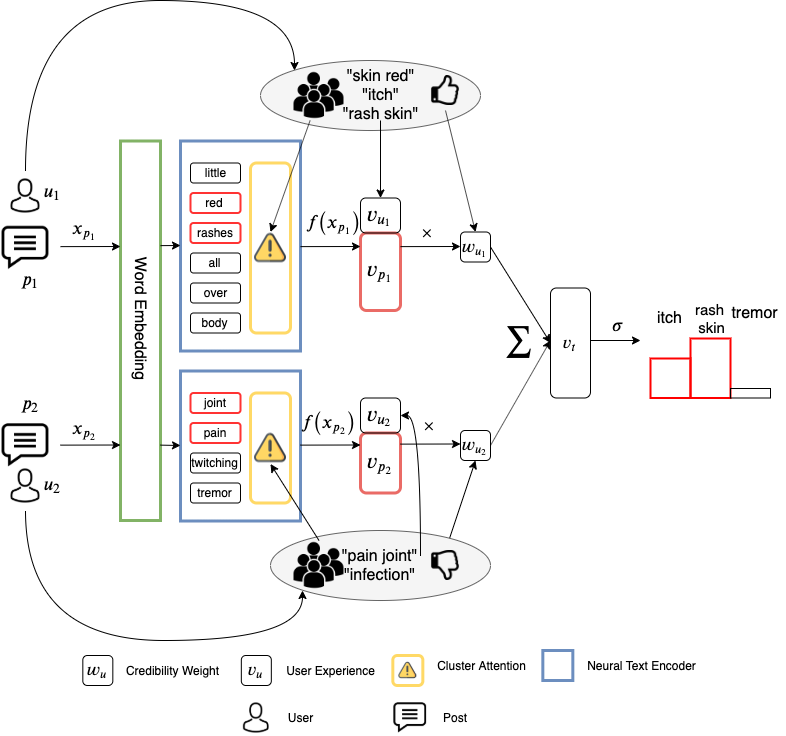
\includegraphics[scale=0.4]{neat.png}
    %Kaz2: It is better to add some words not just "NEAT". 
    \caption{The neural architecture of our proposed NEAT. The blue boxes \\ denoted general text encoders with attention. \\ The highlighted words in red denoted the text segments that are being \\ attended by the encoder. The yellow oval denotes contextual information of \\ User Experience (UE), Credibility Weight (CW) and Cluster Attention (CA).}
    \label{fig:NEAT}
\end{figure}
\pagebreak
\begin{figure}[h]
    \centering
    \captionsetup{justification=centering}
    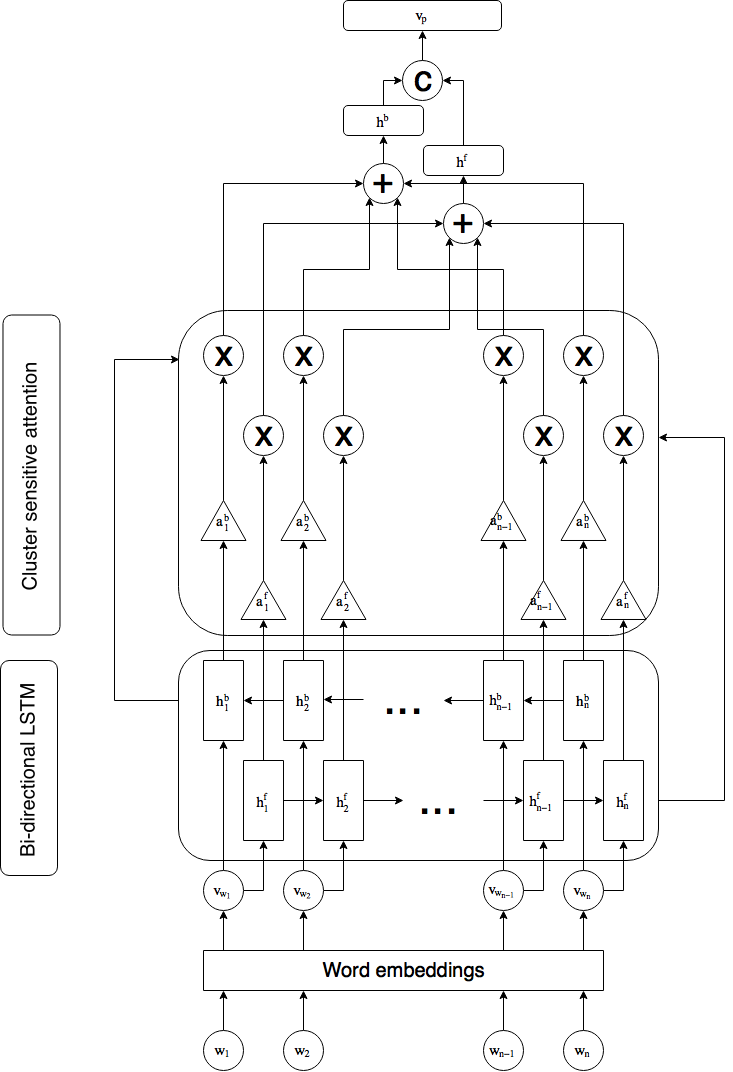
\includegraphics[scale=0.4]{lstm.png}
    \caption{LSTM-based encoder with cluster attention.}
    \label{fig:RNNEncoders}
\end{figure}
\pagebreak
\begin{figure}[h]
    \centering
    \captionsetup{justification=centering}
    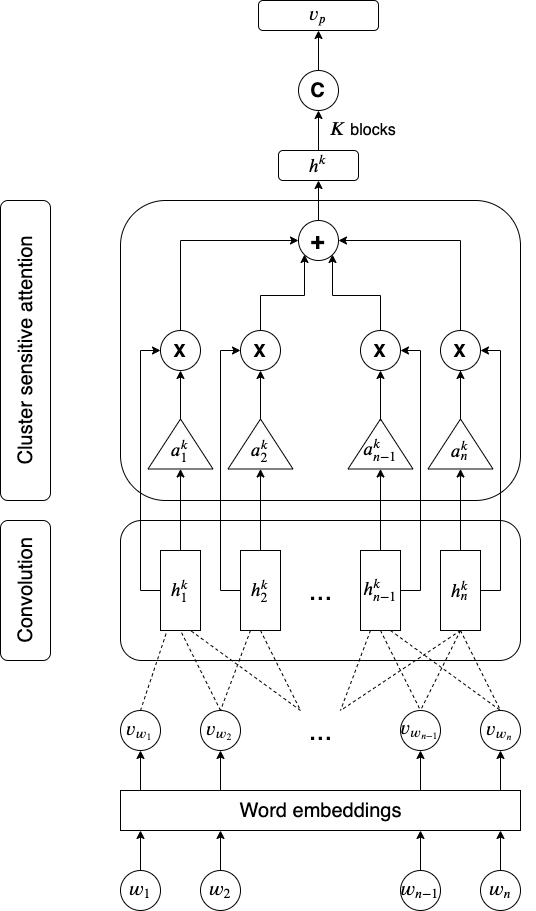
\includegraphics[scale=0.4]{cnn.png}
    \caption{CNN-based Encoder with Cluster Attention}
    \label{fig:CNNEncoders}
\end{figure}
\pagebreak
\begin{figure}[h]
    \centering
    \captionsetup{justification=centering}
    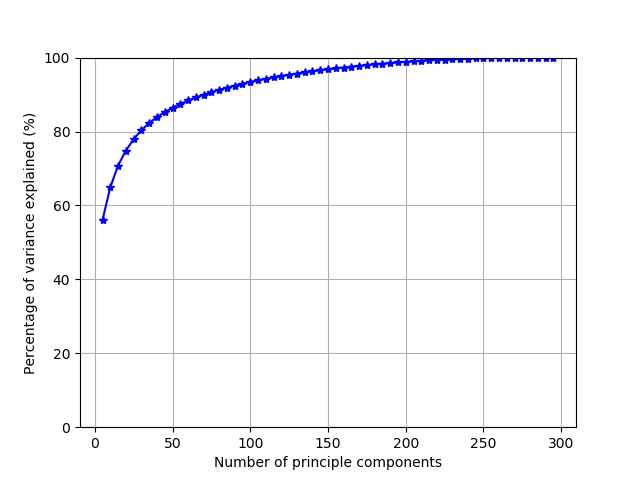
\includegraphics[scale=0.5]{pca.png}
    \caption[Principal Component Analysis]{Principal component analysis.}
    \label{fig:PCA}
\end{figure}
\begin{figure}[h]
    \centering
    \captionsetup{justification=centering}
    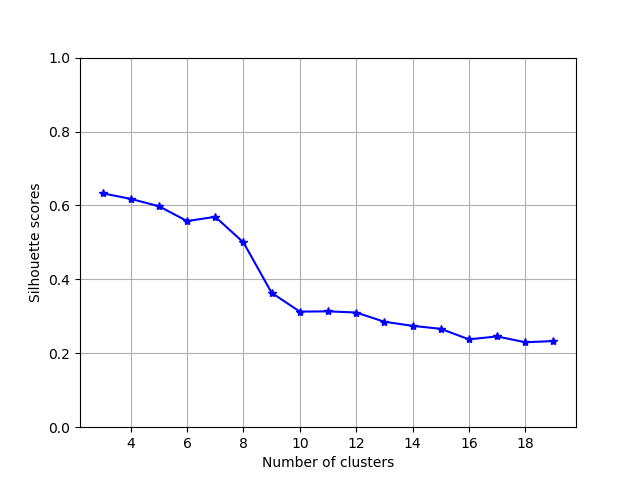
\includegraphics[scale=0.5]{k_means.png}
    \caption[Silhouette scores for user clustering]{Silhouette scores for User Clustering.}
    \label{fig:KMeans}
\end{figure}
% % %%%%%%%%%%%%%%%%%%%%%%%%%%%%%%%%%%%
% % %%                               %%
% % %% Tables                        %%
% % %%                               %%
% % %%%%%%%%%%%%%%%%%%%%%%%%%%%%%%%%%%%

% % %% Use of \listoftables is discouraged.
% % %%
\pagebreak
\section*{Tables}
\begin{table}[h!]
  \centering
  \captionsetup{justification=centering}
  \footnotesize
  \begin{tabular}{|c||p{10.5cm}|}
    \hline
    Drugs & Side effects \\ \hline \hline
    Lexapro & chills, constipation, cough, decreased appetite, \textbf{decreased sexual desire}, \textbf{diarrhea}, \textbf{dry mouth}, joint pain, muscle ache, tingling feeling, \textbf{sleepiness or unusual drowsiness}, unusual dream, \textbf{sweating}, ... \\ \hline
    Xanax &  abdominal or stomach pain, muscle weakness
      , \textbf{changed behavior}, chills, cough, decreased appetite, decreased urine, \textbf{diarrhea}, difficult bowel movement, cough, \textbf{dry mouth}, tingling feeling, \textbf{sleepiness or unusual drowsiness}, slurred speech, sweating, yellow eye... \\ \hline
    Zoloft &  \textbf{changed behavior}, decreased sexual desire, \textbf{diarrhea}, \textbf{dry mouth}, heartburn, \textbf{sleepiness or unusual drowsiness}, \textbf{sweating}... \\ \hline
  \end{tabular}
  % Min: need to indicate what the bolding is for.  Please check.
  % Hoang: noted with thanks
  \caption{Side effects of anti-depressants extracted from a drug -- side effect database. Side effects in common among those listed are bolded.} \label{table:anti_depressant_side_effects}
\end{table}
\begin{table}[h!]
  \centering
  \captionsetup{justification=centering}
  \footnotesize
  %	\resizebox{\textwidth}{!}{%
  \begin{tabular}{|c||p{7cm}|p{1cm}|p{2cm}|}
    \hline
	User ID & Post & Drug mentioned & Aggregated side effects\\ \hline \hline
	3690 & While my experience of 10 years is with Paxil, I expect that Zoloft will be the same. You should definitely feel better within 2 weeks. One way I found to make it easier to sleep was to get lots of exercize. Walk or run or whatever to burn off that anxiety. & \multirow{2}{*}{Zoloft} & changed behavior, decreased sexual desire, diarrhea, dry mouth, heart-  \\ \cline{1-2}
        26521 & I've heard of people going ``cold turkey'' and having withdrawal at 6 months! Please, get in contact with a doctor ASAP! ``common symptoms include dizziness, electric shock-like sensations, sweating, nausea, insomnia, tremor, confusion, nightmares and vertigo'' &  & burn, sleepiness or unusual drowsiness,... \\ \hline
  \end{tabular} 
  \caption{A sample thread, including its list of post--user pairs, mentioned drugs, and side effects.}
  \label{table:sample_thread}
\end{table}
\begin{table}[h!]
    \centering
    \begin{tabular}{|c|c|} \hline
        Cluster & Most common experienced side effects \\ \hline \hline
        $c_{1}$ & vision blurred, yellow skin, vision double, yellow eye, nose stuffy \\ \hline
        $c_{2}$ & headache, itch, stomach pain, weak, nausea \\ \hline
        $c_{3}$ & itch, irritate, headache, pain abdominal, "stomach cramp" \\ \hline
        $c_{4}$ & bad taste, nausea, tiredness, irritate, mouth ulcer \\ \hline
        $c_{5}$ & skin red, itch, rash skin, skin peeling, "burning skin" \\ \hline
        $c_{6}$ & sneezing, nose runny, nose stuffy, decrease sexual desire, pain breast \\ \hline
        $c_{7}$ & nausea, stomach pain, vomit, diarrhea, pain abdominal \\ \hline
    \end{tabular}
    \caption{Most common experienced side effects for each user cluster $c_{i}$ ($i=1$ to $7$).}
    \label{table:cluster_results}
\end{table}
\begin{table}[h!]
    \centering
    \begin{tabular}{|c|c|} \hline
        \# Users & 14,966 \\ \hline
        \# Threads & 78,213 \\ \hline
        Avg. \# of words per post & 67.45 \\ \hline
        Avg. \# of posts per thread & 3.97 \\ \hline
        Avg. \# of participated threads per user & 54.7 \\ \hline
        \# Side effects (SE) & 315 \\ \hline
        Avg. \# of SEs per thread & 74.25 \\ \hline
        \# Drugs & 1869 \\ \hline
        Avg. \# of experienced side effects per user & 128.12 \\ \hline
    \end{tabular}
    %\caption{Dataset statistics.}
    \caption{Some statistics on our dataset.}
    \label{table:dataset_statistics}
\end{table}
\begin{table}[h!]
  \captionsetup{justification=centering}
  \centering
  \scalebox{1.2}
  \footnotesize
  %\scriptsize
  \begin{tabular}{l||c|c|c||c|c|c}
    \hline
    \textbf{System}& \multicolumn{3}{c||}{\centering{Components}} & \multicolumn{3}{c}{\centering{Evaluation Metrics}} \\
    & CW & UE & CA & Pre. & Rec. & $F_1$ \\ \hline \hline
    LSTM-Vanilla   &          &          &           & 0.6173 & 0.407 & 0.4335 \\ \hline
    LSTM-WPE       &\checkmark&          &           & \textbf{0.6376} & 0.4344 & 0.4503 \\ \hline
    LSTM-WPEU      &\checkmark&\checkmark&           & 0.6064 & 0.5001 & 0.4896  \\ \hline
    LSTM-NEAT      &\checkmark&\checkmark&\checkmark & 0.6197 & \textbf{0.5134} & \textbf{0.5064} \\ \hline\hline
    CNN-Vanilla   & & & &  0.7214 & 0.5503 & 0.5637  \\ \hline
    CNN-WPE        &\checkmark&          &           & \textbf{0.7423} & 0.5799 & 0.5804 \\ \hline
    CNN-WPEU       &\checkmark&\checkmark&           & 0.6923 & 0.6350 & 0.5910  \\ \hline
    CNN-NEAT       &\checkmark&\checkmark&\checkmark & 0.7066 & \textbf{0.6431} & \textbf{0.6139} \\ \hline\hline
  \end{tabular}
  \caption{Experimental results obtained by both CNN-based NEAT and LSTM-based NEAT.  In the ``Component'' columns, ``CW'', ``UE'', ``CA'' denote ``Credibility Weights'', ``User Expertise'' and ``Cluster Attention module components'', respectively.}\label{table:Exp}
\end{table}
\begin{table}[h!]
  \captionsetup{justification=centering}
  \centering
  \scalebox{2}
  \footnotesize
  %\scriptsize
  \begin{tabular}{l||c||c||c}
    \hline
    \textbf{Method}& Thread nDCG@2 & Thread Spearman & Forum Spearman \\\hline \hline
    Random  & 0.7968 & -0.0271 & 0.0 \\ \hline
    Post frequency & 0.8812 & 0.4223 & 0.1924 \\ \hline
    Question frequency & 0.8341 & 0.1773 & 0.0279 \\ \hline
    NEAT's Credibility & \textbf{0.8856} & \textbf{0.4403} & \textbf{0.3055} \\ \hline\hline
  \end{tabular}
  \caption{Analysis of NEAT's output user scores in approximating credibility proxy.}\label{table:credibility}
\end{table}
\begin{table}[h!]
  \captionsetup{justification=centering}
  \centering
  \scalebox{1.2}
  \footnotesize
  \begin{tabular}{l||c|c|c|c|c|c|c|c|c}
    \hline
    \textbf{Method}& 
    \multicolumn{3}{c|}{\centering{Ibuprofen}} & \multicolumn{3}{c|}{\centering{Levothyroxine}} & \multicolumn{3}{c}{\centering{Metoformin}}\\
    & Pre. & Rec. & $F_1$ & Pre. & Rec. & $F_1$ & Pre. & Rec. & $F_1$ \\ \hline \hline
    RF & 0.583 & 0.414 & 0.474 & 0.319 & 0.401 & 0.347 & 0.48 & 0.647 & 0.491 \\ \hline
    uNEAT & 0.859 & 0.371 & 0.487 & 0.505 & 0.349 & 0.404 & 0.798 & 0.361 & 0.497 \\ \hline
    NEAT & 0.845 & 0.427 & \textbf{0.536} & 0.549 & 0.385 & \textbf{0.443} & 0.814 & 0.365 & \textbf{0.504} \\ \hline
  \end{tabular}
  \caption{Performance of NEAT against Random Forest (RF) and user permutation (uNEAT) in side effect discovery of Ibuprofen, Levothyroxine, and Metoformin.}\label{table:se_discovery1}
\end{table}
\begin{table}[h!]
  \captionsetup{justification=centering}
  \centering
  \scalebox{1.2}
  \footnotesize
  \begin{tabular}{l||c|c|c|c|c|c}
    \hline
    \textbf{Method} &
    \multicolumn{3}{c|}{\centering{Omeprazole}} &
    \multicolumn{3}{c}{\centering{Alprazolam}}\\
    & Pre. & Rec. & $F_1$ & Pre. & Rec. & $F_1$ \\ \hline \hline
    RF & 0.229 & 0.458 & 0.271 & 0.639 & 0.432 & 0.511 \\ \hline
    uNEAT & 0.534 & 0.393 & 0.394 & 0.981 & 0.551 & 0.663 \\ \hline
    NEAT & 0.522 & 0.421 & \textbf{0.41} & 0.977 & 0.596 & \textbf{0.704} \\ \hline
  \end{tabular}
  \caption{Performance of NEAT against Random Forest (RF) and user permutation (uNEAT) in side effect discovery of Omeprazole and Alprazolam.}\label{table:se_discovery2}
\end{table}
\begin{table}[h!]
  \captionsetup{justification=centering}
  \centering
  \scalebox{1.2}
  \footnotesize
  \begin{tabular}{l||c|c|c|c|c}
    \hline
    \textbf{Method} & Ibuprofen & Levothyroxine & Metoformin & Omeprazole & Alprazolam \\ \hline \hline
    UMLS Tagging & 0.6801 & 0.6145 & 0.8378 & \textbf{0.5218} & 0.614 \\ \hline
    Neural Extractor~\cite{ding2018attentive} & 0.6741 & 0.6259 & 0.8092 & 0.4665 & 0.6161 \\ \hline
    NEAT's Attention & \textbf{0.7073} & \textbf{0.7119} & \textbf{0.8557} & 0.504 & \textbf{0.688} \\ \hline
  \end{tabular}
  \caption{Precision of NEAT's Attention mechanism against baselines in mentioned side effect extraction.}\label{table:se_extraction}
\end{table}
\begin{table}[h!]
  \captionsetup{justification=centering}
  \centering
  \scalebox{1.2}
  \footnotesize
  \begin{tabular}{c|p{3cm}|p{7cm}}
    \hline
    User id & Cluster's side effects & Post content \\ \hline \hline
    8420 & stomach pain, headache, itch, weak, nausea & I won\'t commit suicide but the \textcolor{blue}{discomfort} $<$U$>$ is enough to make me want to die right now [...] I feel like I have sever Akathisia (inner \textcolor{red}{restlessness}$<$U,X$>$ that makes you feel like your body is electrified [...] I also have \textcolor{blue}{nausea}$<$U,X,N$>$, but I can eat a little, \textcolor{blue}{sweating}$<$U,X,N$>$/cold, and extreme \textcolor{red}{fatigue}$<$U,X$>$, although I already have chronic fatigue [...] I also get \textcolor{blue}{anxious}$<$U,X,N$>$ if I take more oxycodone for breakout \textcolor{red}{pain}$<$U$>$ and then go right \textcolor{red}{back}$<$U$>$ down \\ \hline
  \end{tabular}
  \caption{A test example highlighting the extracted correct (blue) and wrong (red) side effects wrapped in $<>$ by UMLS Tagging (U), Neural Extractor (X) and NEAT's Attention (N)}\label{table:extraction_ex}
\end{table}
\begin{table}[h!]
  \captionsetup{justification=centering}
  \centering
  \scalebox{1.2}
  \footnotesize
  %\scriptsize
  \begin{tabular}{l||c|c|c||c|c|c}
    \hline
    \textbf{System}& \multicolumn{3}{c||}{\centering{Components}} & \multicolumn{3}{c}{\centering{Evaluation Metrics}} \\
    & CW & UE & CA & Pre. & Rec. & $F_1$ \\ \hline \hline
    LSTM-UE   &          & \checkmark &           & 0.6513 & 0.4204 & 0.4531 \\ \hline
    LSTM-CA       & &          & \checkmark & 0.6416 & 0.4293 & 0.4611 \\ \hline\hline
    CNN-UE   &  & \checkmark & &  0.6738 & 0.6185 &  0.5743  \\ \hline
    CNN-CA        & &          & \checkmark & 0.7441 & 0.5616 & 0.5883 \\ \hline\hline
  \end{tabular}
  \caption{Algorithm performance for individual integration of UE and CA.}\label{table:individual}
\end{table}
% % \begin{table}[h!]
% % \caption{Sample table title. This is where the description of the table should go.}
% %       \begin{tabular}{cccc}
% %         \hline
% %           & B1  &B2   & B3\\ \hline
% %         A1 & 0.1 & 0.2 & 0.3\\
% %         A2 & ... & ..  & .\\
% %         A3 & ..  & .   & .\\ \hline
% %       \end{tabular}
% % \end{table}

\pagebreak
%%%%%%%%%%%%%%%%%%%%%%%%%%%%%%%%%%%
%%                               %%
%% Additional Files              %%
%%                               %%
%%%%%%%%%%%%%%%%%%%%%%%%%%%%%%%%%%%
% \section*{Additional Files}
%   \subsection*{Additional file 1 --- Sample additional file title}
%     Additional file descriptions text (including details of how to
%     view the file, if it is in a non-standard format or the file extension).  This might
%     refer to a multi-page table or a figure.

%   \subsection*{Additional file 2 --- Sample additional file title}
%     Additional file descriptions text.


\end{backmatter}
\end{document}
